\documentclass[10pt]{beamer}



%%%
% PREAMBLE FOR THIS DOC 
%%%
%https://tex.stackexchange.com/questions/68821/is-it-possible-to-create-a-latex-preamble-header
\usepackage{/Users/miw267/Repos/csci246_spring2025/slides/preambles/beamer_preamble_for_CSCI246}

\usepackage{wrapfig}  


%%% TRY TO RESHOW TOC AT EACH SECTION START (with current section highlighted)
% Reference: https://tex.stackexchange.com/questions/280436/how-to-highlight-a-specific-section-in-beamer-toc
\newcommand\tocforsect[2]{%
  \begingroup
  \edef\safesection{\thesection}
  \setcounter{section}{#1}
  \tableofcontents[#2,currentsection]
  \setcounter{section}{\safesection}
  \endgroup
}


\usepackage[normalem]{ulem} % for strikeout (\sout)

%%%% HERES HOW TO DO IT CORRECTLY
% FIRST IN .STY FILE, DO
%\usetheme[sectionpage=none]{metropolis}
% THEN AT EACH SECTION DO
%\begin{frame}{Outline}
%  \tableofcontents[currentsection]	
%\end{frame}



%\setbeamertemplate{navigation symbols}{}
%\setbeamertemplate{footline}[frame number]{}


%%%
% DOCUMENT
%%%

\begin{document}

%\maketitle

%% Title page frame
%\begin{frame}
%    \titlepage 
%\end{frame}



\title{02/26/2026: Stochastic Calculus}
\author{CSCI 546: Diffusion Models}
\date{Textbook reference: Chang Sec 6.7-6.8, GS Sec  13.7}

\begin{frame}
    \titlepage 
\end{frame}

\begin{frame}

\begin{mygreenbox}[title=Announcement (Sign-in Sheet)]
Please sign the sign-in sheet.
\end{mygreenbox}

\vfill 


%\begin{myyellowbox}[title=Agenda]
%\begin{enumerate}
%	\item ($\approx$ 10 mins) Notes on Midterm Exam
%	\item  ($\approx$ 10 mins) Review Problem Set \#11
%	\item  ($\approx$ 10 mins) Mini-lecture
%	\item ($\approx$ 25 mins) Group Exercises
%	\item ($\approx$ 20 mins) Briefing on Backward Equation
%\end{enumerate}
%
%\end{myyellowbox}
	
\end{frame}

\begin{frame}[standout]
Review Problem Set \#12
\end{frame}

\begin{frame}[standout]
Concepts for Problem Set \#13
\end{frame}


\begin{frame}[standout]
Outline for today's material
\begin{itemize}
\item \textbullet \quad \alert{Interpreting a Stochastic Differential Equation (SDE)}
\item \textbullet \quad Difficulties with Integrating Against Brownian Motion
\end{itemize}

\end{frame}

\begin{frame}{Stochastic Differential Equations}

A diffusion process $X$ with drift coefficient $\mu(x,t)$ and diffusion coefficient $\sigma(x,t)$ can be expressed as
\[ dX = \mu(X,t) dt + \sigma(X,t) dW, \]
where $W$ is standard Brownian motion. 
\vfill
\pause 
This is known as a \alert{Stochastic Differential Equation} (SDE).  \pause 
Our goal over the next two meetings is to make sense of SDEs.
\end{frame}

\begin{frame}{Discretized SDEs}

\fbox{%
\begin{minipage}{\linewidth}
\colorbox{blue!30}{\textbf{Definition.}} A SDE for the diffusion process $X$ with drift coefficient $\mu(x,t)$ and diffusion coefficient $\sigma(x,t)$ is
\[ dX = \mu(X,t) dt + \sigma(X,t) dW, \]
where $W$ is standard Brownian motion. 
\end{minipage}
	
}
\vfill

\only<2>{\colorbox{yellow!30}{\textbf{Poll.}} We've already seen one way to make sense of these.  What is it?}

\only<3-6>{\colorbox{red!30}{\textbf{Discretized SDE's}} We've already seen (Chang Sec 6.1) that we can generate a solution to a discretized SDE via} \only<3>{\alert{how???}} 
\only<4-6>{
%
	\begin{align*}
	 \Delta X = \mu(X_t,t) \Delta t + \sigma(X_t,t) \, \sqrt{\Delta t} \, Z  \qquad Z \sim N(0,1)
	\end{align*}
%
} 

\only<5-6>{\colorbox{yellow!30}{\textbf{Poll.}} What's going on with then second summand? For instance, why is the second $\Delta t$ under a square root?}

\only<6>{\colorbox{green!30}{\textbf{Solution.}} 

\begin{align*}
\begin{cases}
W \sim N(0,t)& \\
\text{indep. increments} & 	
\end{cases}
\implies 
\Delta W \sim N(0,\Delta t) =
\sqrt{\Delta t} N(0,1)
\end{align*}
}
	
\end{frame}


\begin{frame}{SDE as continuous-time random walk}

Conceptually, a SDE is a continuous-time limit of a random walk (with state-dependent drift and variance).

\pause 
\vfill 
Consider

\[ X_{k+1} = X_k 
+
\mu(X_k)\,\Delta t
+
\sigma(X_k)\,\Delta W_k,
\]

where

\[\Delta W_k \sim \mathcal N(0,\Delta t). \]

\vfill 
\pause 
This is just a random walk whose:

\begin{itemize}
\item mean step size = $ \mu(X_k)\Delta t $
\item variance of step = $ \sigma^2(X_k)\Delta t $
\end{itemize}

\vfill 
\pause 

As $\Delta t \to 0$, this converges (under standard conditions) to the SDE

\[ dX_t = \mu(X_t) \, dt + \sigma(X_t)\,dW_t \]


\end{frame}
	


\begin{frame}{SDE: Shorthand for an integral equation}

In general, we have
\only<1>{\[ dX = \mu(X,t) dt + \sigma(X,t) dW \]}
\only<2-4>{
\[
dX
=
\underbrace{
\colorbox{green!20}{$\mu(X,t)\,dt$}
}_{\text{\color{green!70!black}deterministic drift}}
\;+\;
\underbrace{
\colorbox{red!20}{$\sigma(X,t)\,dW$}
}_{\text{\color{red!70!black}random diffusion}}
\]
}

\only<3-4>{Really, this is a shorthand for the integral equation}

\only<3>{
\[ \int dX(t) = \int \mu(X,t) dt +  \int \sigma(X,t) dW(t) \]
}

\only<4>{
\[
\int dX(t)
=
\underbrace{
\colorbox{green!20}{$\int \mu(X,t)\,dt$}
}_{\text{\color{green!70!black} Riemann integral \greencheck }}
\;+\;
\underbrace{
\colorbox{red!20}{$\int \sigma(X,t)\,dW(t)$}
}_{\text{\color{red!70!black} ??? }}
\]
}
\end{frame}


\begin{frame}[standout]
Outline for today's material
\begin{itemize}
\item \textbullet \quad Interpreting a Stochastic Differential Equation (SDE)
\item \textbullet \quad \alert{Difficulties with Integrating Against Brownian Motion}
\end{itemize}

\end{frame}

\begin{frame}{}

\begin{center}

\includegraphics[width=.9\textwidth]{images/homer.png}
\end{center}
\vfill \pause 
Similarly, the difficulty with (and solution to) integrating $\int f(t) \,dW(t)$	 lies with the notion of the \alert{variation of a function}.
\end{frame}


\begin{frame}{Total variation of a function}
\begin{center}
First, form a \textbf{dyadic partition} of $[0,t]$ by chopping it into $2^n$ bins. 

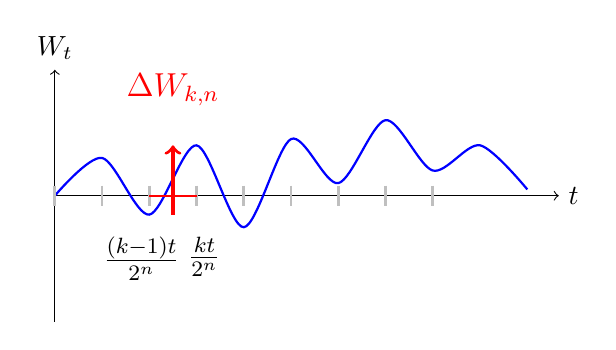
\begin{tikzpicture}[scale=0.8]

% -------- PARAMETERS --------
\def\tmax{6}              % length of time axis
\def\nlevel{3}            % n (so number of bins = 2^n)
\pgfmathsetmacro{\nbins}{2^\nlevel}
\pgfmathsetmacro{\dt}{\tmax/\nbins}

% -------- AXES --------
\draw[->] (0,0) -- (\tmax+2,0) node[right] {$t$};
\draw[->] (0,-2) -- (0,2) node[above] {$W_t$};


% -------- BROWNIAN PATH (aligned with dyadic partitions) --------
% Dyadic bins: 2^n
\def\tmax{6}
\def\nlevel{3}
\pgfmathsetmacro{\nbins}{2^\nlevel}
\pgfmathsetmacro{\dt}{\tmax/\nbins}

% Define path coordinates exactly at partition points
% y-values chosen for illustration
\coordinate (P0) at (0,0);
\coordinate (P1) at (\dt,0.6);           % t = dt
\coordinate (P2) at (2*\dt,-0.3);        % t = 2*dt
\coordinate (P3) at (3*\dt,0.8);         % t = 3*dt
\coordinate (P4) at (4*\dt,-0.5);
\coordinate (P5) at (5*\dt,0.9);
\coordinate (P6) at (6*\dt,0.2);
\coordinate (P7) at (7*\dt,1.2);
\coordinate (P8) at (8*\dt,0.4);
\coordinate (P9) at (9*\dt,0.8);
\coordinate (P10) at (10*\dt,0.1);       % last point (t = tmax)

% Draw smooth Brownian path through these coordinates
\draw[thick,blue] plot[smooth] coordinates {
  (P0) (P1) (P2) (P3) (P4) (P5) (P6) (P7) (P8) (P9) (P10)
};

% -------- DYADIC PARTITION LINES --------
\foreach \k in {0,...,\nbins} {
    \pgfmathsetmacro{\x}{\k*\dt}
     \draw[gray!50, line width=1pt]  (\x,0.16) -- (\x,-0.16);
}

% -------- HIGHLIGHT ONE INTERVAL (vertical arrow) --------
\pgfmathsetmacro{\kexample}{3}
\pgfmathsetmacro{\xleft}{(\kexample-1)*\dt}
\pgfmathsetmacro{\xright}{\kexample*\dt}
\pgfmathsetmacro{\xmid}{(\xleft+\xright)/2}  % midpoint of bin

% Get the y-value at the left endpoint (or midpoint) for starting the arrow
\coordinate (Ybase) at (\xmid,-0.3);     %arrow start
\coordinate (Ytop)  at (\xmid,0.8);   % arrow goes straight up

% Draw vertical arrow
\draw[red,very thick,->] (Ybase) -- (Ytop) 
    node[midway, above, yshift=8mm] {\large $\Delta W_{k,n}$};

% Draw horizontal red line under the bin
\draw[red,thick] (\xleft,0) -- (\xright,0);

% Optional: dashed lines connecting bin ends to curve (not needed for vertical arrow)
% \draw[red,dashed] (\xleft,0) -- (Yleft);
% \draw[red,dashed] (\xright,0) -- (Yright);

% Label partition points
\node[below, yshift=-4mm, xshift=-1mm] at (\xleft,0) {\large $\frac{(k-1)t}{2^n}$};
\node[below, yshift=-4mm, xshift=+1mm] at (\xright,0) {\large $\frac{kt}{2^n}$};

\end{tikzpicture}
\vfill 
\pause 

\alert{Total variation over a partition}:
\[
T_n = \sum_{k=1}^{2^n} |\Delta W_{k,n}|
\]


\alert{Total variation}: $\lim_{n \to \infty} T_n$

\end{center}
\end{frame}




\begin{frame}{Brownian Motion has \alert{infinite} total variation}


\begin{mygreenbox}[title=Theorem]
Standard Brownian motion has infinite total variation over any interval $[0,T]$ where $T>0$. 
\end{mygreenbox}

\vfill 
\pause 
\colorbox{yellow!30}{\textbf{Poll.}} So who cares?! 
\pause 
\bottomtext{\hfill Reference: Gautam Iyer, \textit{\href{https://www.math.cmu.edu/~gautam/sj/teaching/2021-22/944-scalc-finance1/pdfs/ch3-int.pdf}{\underline{\blue{Stochastic Integration. (Lecture notes.)}}}}}
\end{frame}












\begin{frame}{What's wrong with infinite total variation?}

It means we can't use normal tools to integrate $\int f(t) \,dW(t)$!

\vfill 
 	
\only<2>{
\begin{myyellowbox}[title=Definition]
The \textbf{Riemann integral} of a smooth function $f(t)$ on $[0,T]$ is given by
\[\int_0^T f(t) \, dt = \lim_{||P|| \to 0} \sum_{i=1}^n f(t_i^*)(t_i - t_{i-1}) \]
where $P = \set{0 = t_0 < t_1 < \hdots < t_n = T}$ is a partition of $[0, T]$, $||P|| = \max\set{t_{i+1} - t_{i}}$, and $t_{i-1} \leq t_i^* \leq t_i$.
\end{myyellowbox}
}


\only<3->{
\begin{myyellowbox}[title=Definition]
The \textbf{Riemann-Stieljes integral} integrates a function f(t) with respect to another function $\red{g}(t)$.  It is defined using the following sum:
\[\int_0^T f(t) \, d\red{g}(t) = \lim_{||P|| \to 0} \sum_{i=1}^n f(t_i^*)(\red{g}\big(t_i) - \red{g}(t_{i-1})\big) \]
where $P = \set{0 = t_0 < t_1 < \hdots < t_n = T}$ is a partition of $[0, T]$, $||P|| = \max\set{t_{i+1} - t_{i}}$, and $t_{i-1} \leq t_i^* \leq t_i$.
\end{myyellowbox}
}

\vfill 
\only<4->{
\begin{myredbox}[title=The problem] We'd like to use the above scheme, but for it to work directly, we need $g$ to have \textbf{finite total variation}!
\end{myredbox}	
}
\vfill 
\only<5->{
\bottomtext{\hfill Reference: Gautam Iyer, \textit{\href{https://www.math.cmu.edu/~gautam/sj/teaching/2021-22/944-scalc-finance1/pdfs/ch3-int.pdf}{\underline{\blue{Stochastic Integration. (Lecture notes.)}}}}}}
\end{frame}


\begin{frame}{Quadratic variation to the rescue!}

If we can't use normal tools to integrate $\int f(t) \,dW(t)$, what should we do?

\vfill 
\only<2->{\colorbox{green!30}{\textbf{A lead.}} It turns out that the \alert{quadratic} variation of Brownian motion is almost surely finite.}  

\vfill 
\only<3->{This is the key to constructing the It\^o integral.} 

\end{frame}


\begin{frame}{Quadratic variation of a function}
\begin{center}
First, form a \textbf{dyadic partition} of $[0,t]$ by chopping it into $2^n$ bins. 

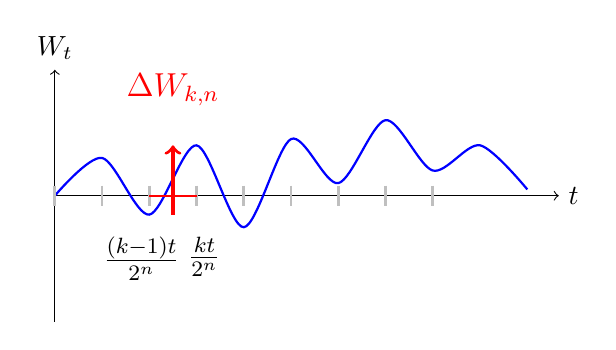
\begin{tikzpicture}[scale=0.8]

% -------- PARAMETERS --------
\def\tmax{6}              % length of time axis
\def\nlevel{3}            % n (so number of bins = 2^n)
\pgfmathsetmacro{\nbins}{2^\nlevel}
\pgfmathsetmacro{\dt}{\tmax/\nbins}

% -------- AXES --------
\draw[->] (0,0) -- (\tmax+2,0) node[right] {$t$};
\draw[->] (0,-2) -- (0,2) node[above] {$W_t$};


% -------- BROWNIAN PATH (aligned with dyadic partitions) --------
% Dyadic bins: 2^n
\def\tmax{6}
\def\nlevel{3}
\pgfmathsetmacro{\nbins}{2^\nlevel}
\pgfmathsetmacro{\dt}{\tmax/\nbins}

% Define path coordinates exactly at partition points
% y-values chosen for illustration
\coordinate (P0) at (0,0);
\coordinate (P1) at (\dt,0.6);           % t = dt
\coordinate (P2) at (2*\dt,-0.3);        % t = 2*dt
\coordinate (P3) at (3*\dt,0.8);         % t = 3*dt
\coordinate (P4) at (4*\dt,-0.5);
\coordinate (P5) at (5*\dt,0.9);
\coordinate (P6) at (6*\dt,0.2);
\coordinate (P7) at (7*\dt,1.2);
\coordinate (P8) at (8*\dt,0.4);
\coordinate (P9) at (9*\dt,0.8);
\coordinate (P10) at (10*\dt,0.1);       % last point (t = tmax)

% Draw smooth Brownian path through these coordinates
\draw[thick,blue] plot[smooth] coordinates {
  (P0) (P1) (P2) (P3) (P4) (P5) (P6) (P7) (P8) (P9) (P10)
};

% -------- DYADIC PARTITION LINES --------
\foreach \k in {0,...,\nbins} {
    \pgfmathsetmacro{\x}{\k*\dt}
     \draw[gray!50, line width=1pt]  (\x,0.16) -- (\x,-0.16);
}

% -------- HIGHLIGHT ONE INTERVAL (vertical arrow) --------
\pgfmathsetmacro{\kexample}{3}
\pgfmathsetmacro{\xleft}{(\kexample-1)*\dt}
\pgfmathsetmacro{\xright}{\kexample*\dt}
\pgfmathsetmacro{\xmid}{(\xleft+\xright)/2}  % midpoint of bin

% Get the y-value at the left endpoint (or midpoint) for starting the arrow
\coordinate (Ybase) at (\xmid,-0.3);     %arrow start
\coordinate (Ytop)  at (\xmid,0.8);   % arrow goes straight up

% Draw vertical arrow
\draw[red,very thick,->] (Ybase) -- (Ytop) 
    node[midway, above, yshift=8mm] {\large $\Delta W_{k,n}$};

% Draw horizontal red line under the bin
\draw[red,thick] (\xleft,0) -- (\xright,0);

% Optional: dashed lines connecting bin ends to curve (not needed for vertical arrow)
% \draw[red,dashed] (\xleft,0) -- (Yleft);
% \draw[red,dashed] (\xright,0) -- (Yright);

% Label partition points
\node[below, yshift=-4mm, xshift=-1mm] at (\xleft,0) {\large $\frac{(k-1)t}{2^n}$};
\node[below, yshift=-4mm, xshift=+1mm] at (\xright,0) {\large $\frac{kt}{2^n}$};

\end{tikzpicture}
\vfill 
\pause 

\alert{Quadratic variation over a partition}:
\[
Q_n = \sum_{k=1}^{2^n} (\Delta W_{k,n})^2
\]


\alert{Quadratic variation}: $\lim_{n \to \infty} Q_n$

\end{center}
\end{frame}

\begin{frame}{\alert{Quadratic} variation to the rescue!}

The quadratic variation of Brownian motion is almost surely finite.
\vfill 

\only<2->{
\begin{mygreenbox}[title=Theorem (Chang 6.7)]
Let $Q$ be the quadratic variation of standard Brownian motion over interval $[0,t]$. Then $Q=t$ with probability 1. 
\end{mygreenbox}
}
\vfill 

\only<3->{This is the key step in constructing the It\^o integral.} \only<4->{In essence, this relation reflects the strange scaling of space and time.
\[ (dW)^2 \approx dt\]	
}

\vfill 
\only<5->{That is, the square of an infinitesimal Brownian increment is of order $dt$.}


\only<6->{\colorbox{yellow!30}{\textbf{Poll.}} Where does this strange relationship come from?}


\end{frame}


\begin{frame}{Let's Revisit: Brownian Motion as the continuous time limit of a Random Walk}
\footnotesize 
\textbf{Discrete model}

\only<1->{
\[
X_n = \sum_{k=1}^n \xi_k,
\qquad
\xi_k =
\begin{cases}
+\Delta x & \text{w.p. } \tfrac12 \\
-\Delta x & \text{w.p. } \tfrac12
\end{cases}
\]

Time after $n$ steps:
\[
t = n \Delta t
\]

\vspace{0.5em}
}

\only<2->{
\textbf{Variance scaling}

\[
\mathrm{Var}(X_n) = n (\Delta x)^2
\]
}
\only<3>{\colorbox{yellow!30}{\textbf{Poll.}} (Why does the above equation hold?)}
\only<4->{
Since $n = \dfrac{t}{\Delta t}$,

\[
\mathrm{Var}(X_n)
=
\frac{t}{\Delta t} (\Delta x)^2
=
t \, \frac{(\Delta x)^2}{\Delta t}.
\]
}
\medskip
\only<5->{
\textbf{Requirement}

To obtain a finite, non-trivial limit as 
$\Delta x, \Delta t \to 0$, we require
\[
\boxed{\frac{(\Delta x)^2}{\Delta t} \to D > 0.}
\]
}
\only<5>{\colorbox{yellow!30}{\textbf{Poll.}} Why do we want a finite, non-trivial limit?}
\end{frame}

\begin{frame}{Looking ahead}
\fbox{%
\begin{minipage}{\linewidth}
\colorbox{blue!30}{\textbf{Definition.}} A SDE for the diffusion process $X$ with drift coefficient $\mu(x,t)$ and diffusion coefficient $\sigma(x,t)$ is
\[ dX = \mu(X,t) dt + \sigma(X,t) dW, \]
where $W$ is standard Brownian motion. 
\end{minipage}
}
\vfill 
Next class, we'll show how to integrate
\[\int \sigma(X,t)\,dW(t)\] 
\pause 
To do so, we'll need a new tool called \alert{It\^{o} Integration.}
\end{frame}

\begin{frame}{Random Groups}

\begin{columns}
\begin{column}{0.33\textwidth}
Aubrey Williams: 5 \\ 
Austin Barton : 7 \\ 
Blake Sigmundstad: 5 \\ 
Diego Moylan: 6 \\ 
Dillon Shaffer: 1 \\ 
Ismoiljon Muzaffarov: 1 \\ 
Jacob Tanner: 8 \\\end{column}
\begin{column}{0.33\textwidth}
Josh Stoneback: 3 \\ 
Joshua Bowen: 2 \\ 
Joshua Culwell: 1 \\ 
Laura Banaszewski: 2 \\ 
Lina Hammel: 6 \\\end{column}
\begin{column}{0.33\textwidth}
Logan Racz: 2 \\ 
Matt Hall: 8 \\ 
Mike Kadoshnikov: 3 \\ 
Owen Cool: 4 \\ 
Racquel Bowen: 4 \\ 
Samuel Mocabee: 3 \\ 
Tatiana Kirillova: 7 \\\end{column}
\end{columns}

\end{frame}



\begin{frame}{Group exercises - Problem Set 12}
\footnotesize  
\begin{enumerate}
	\item (Chang Sec 6.7) \textbf{Quadratic variation of Brownian motion.}. Let $W$ be Brownian motion, and let $\Delta W_{k,n}$ denote the increment 
	\[ \Delta W_{k,n} = W \bigg( \frac{kt}{2^n} \bigg) -  W \bigg( \frac{(k-1)t}{2^n} \bigg)\]  
and let $Q_n = \sum_{k=1}^{2^n} (\Delta W_{k,n})^2$.  Compute $\E[Q_n]$ and $\Var[Q_n]$.
\end{enumerate}


\end{frame}


\end{document}
